\documentclass{article}
\usepackage{graphicx}
\usepackage{amsmath}
\usepackage{amsthm}
\usepackage{amssymb}
\usepackage{geometry}
\usepackage{twemojis}
\usepackage{subcaption}
\usepackage[style=numeric,bibstyle=numeric,backend=biber,natbib=true,maxbibnames=99,giveninits=true,uniquename=init]{biblatex}
\usepackage[utf8]{inputenc}

\addbibresource{../bibliography.bib}

% options: change 'markings' to 'entries'? include 'handwritten'?
\title{Fine-tuned optical character recognition for dental fossil markings}

\begin{document}

\tableofcontents

\section{Abstract}

Digitizing and uniformizing the structure of handwritten fossil catalogues exhibits a great 
potential for increasing the accuracy of paleontological data analysis by increasing sample sizes. 
Approximately 90, 000 of such samples reside in the archives of the National Museum of Kenya, and 
an ongoing effort is to store this data in a digital format for better accessibility.
A previous project utilized a commercial optical character recognition service for automated reading of these catalogues. This generalist
handwriting detection model lacked the ability to detect special characters used to denote tooth samples, and could not utilize prior knowledge 
of the vocabulary that is more likely to be present in the data, leading to loss of information and detection mistakes.

This thesis aims to build a specialist character recognition model to increase the accuracy of 
the bone or tooth type specifying column of the digitized data by fine-tuning a state-of-the-art optical 
character recognition model with few-shot transfer learning. This is performed by first finding most accurate
recognition models, variants of convolutional neural networks or vision transformers, and most successful 
transfer learning methods for adapting a model to a new character set. Then, the character 
recognition accuracy of combinations of these methods are benchmarked using handlabeled image segments from the 
fossil catalogues. The final aim of this work is to use the best-performing model 
to obtain an accurate reading of the catalogues of the National Museum of Kenya, and publish the final model to be used 
by the paleontological community for further digitization efforts.

Keywords: Optical character recognition, Few-shot transfer learning, Paleontological databases

\section{Introduction}


% use 'we' in intro

% outline of an introduction
% introduce the broad research area, why this is interesting. 1-2 paragraphs. context, anyone should be able to understand.
% first sentences: state the topic clearly
% broad research area: paleontology: data analysis on fossil finds
% dig fossil from the ground. identify:which bone,species,time. write this on a field slip, a slice of
% baking sheet like paper 
% analysis: take set of fossils, use methods for deducing eg climate, habitat, vegetation
% why this is interesting 
%     reactions of ecosystems to climate change
%     what ancient worlds were like 
%     how ancient humans lived
%     mass extinction events

The field of paleoecology conducts data analysis on fossil specimens.
Such analysis is always started from the ground: after a fossil specimen has been found, it is 
carefully measured and identified: which bone and species the fragment is from, and how old it is. On site, such information is logged on field slips, small thin sheets of 
paper with a pre-printed form. The analysis has then been traditionally conducted by 
collecting such entries, sometimes collected in handwritten tabular catalogues, and running statistical 
tests on the sample set. With this analysis, facts from distant past, such as climate, habitats and 
vegetation can be deduced \cite{Faith_Lyman_2019}. Syntheses of such results consequently allow us to 
answer larger questions, such as how ecosystems reacted to climate changes, how mass extinction events 
came about, and what the living world could be like \cite{Žliobaitė2023}. Understandably, answering such 
questions has become ever more pressing.

% now we have a stack of baking sheets in a room in kenya.
% paleontologists form all over the world want to solve climate change, among other problems
% big data methods would explode what paleoecology can do
% so we need to put the baking sheets on the computer to do analysis on big data
% what is the topic of my work?
% the baking sheets contain weird characters that a normal reader cannot read.
% my topic is to read them

To find answers to large-scale problems, more sophisticated computational data analysis methods have come about,
relying on large datasets. Due to the infeasibility of collecting stacks of fields slips across sometimes multiple 
continents, specimens residing in archives of institutions have been converted to digital, public databases.
One such institution is the National Museum of Kenya that holds a large fraction of data collected from one 
of the most valuable fossil sites globally, the lake Turkana. The digitization effort was started by
using commercial optical character recognition software, combined with heuristical and machine learning approaches, 
resulting in satisfactory accuracy on conventional handwritten text. However, a large hurdle in the existing 
approach were the special characters used to denote which teeth each specimen contains. The aim of this work is 
to digitize these markings accurately.

% explanation of the specific problem
%given scanned images and data with bounding boxes of sentences and words where tooth denoting words are 
%badly read, how can tooth element recognition results be improved? Goal is to have both this is what the element 
%/ nature of specimen column says (eg example here) and what/which teeth are found in this specimen in standardized format
%(eg example here)
%the topic of my work is creating a tool that inputs cropped images from the sheets containing
%handwritten specifications of fossil bones and outputs what the text says

Specifically, this work uses as input data both scan images of the fossil slips and catalogues, and outputs from the Azure AI Vision software \cite{azurevision}. The existing outputs consist of sentence and word-level readings, along with bounding boxes defining 
the location of each word or sentence. The main research question is the following: 

How, given the input data, can the accuracy of the readings of the tooth markings be improved?

% brief review of standard solutions to this (or related) problem(s) and their limitation in this case (incl. reference key papers)
% TODO, once literature review is done


% outline of the new solution
% TODO, likely: tooth or not classifier -> trocr or tooth classifier -> output concatenation

% how the solution was evaluated, what were the results of this evaluations. scope and limitations
% TODO

% relevance for other work: why was this specific problem? how can this be concretely used?
% relevance of this work: KNM is able to have way more precise dental element markings
% to other catalogues: previous project + this a complete solution to digitizing the handwritten data 
% relevance of this work: any field that does:
% - ocr on unconventional characters
% - ocr where each character has a multivariate output (eg. this is an a. it is underlined could be letter and underlined /not underlined)

The direct impact of this work is an improved precision of the tooth element entries in the digitized 
fossil catalogues of the National Museum of Kenya, but the results are applicable to a wider domain of problems.
Intuitively, the results are directly applicable to other fossil archives using similar notation: only a fine-tuning of the 
models to the new archival data is necessary.
For other handwritten archives, the results presented can be used to improve recognition accuracy, especially in cases 
where the data contains characters other than latin letters or arabic numerals. Additionally, this work presents
a potential solution for when the target character set can be expressed with multivariate output data. This could, for 
instance, be handwriting with occasional underlinings, where the bivariate output could be the letter and a boolean variable for 
whether the character was underlined.

% organization
The rest of this thesis is organized as follows. First, the necessary background theory is 
presented. For deep neural networks, the following concepts are introduced:
the basic network structure, how training is conducted, basic building blocks of character-recognizing network architectures, performance-improving 
heuristics, and transfer learning. For paleoecology, the background covers 
foundational ecological laws followed by a brief introduction to methods used in
paleoenvironmental reconstruction, especially focusing on inferences from tooth data.
As the last background section, the composition of mammal teeth is presented. 
Second, related work is presented, both on
handwritten archive digitization and transfer learning with character-recognizer models.
Next, the experimental setup is introduced, covering dataset creation, labeling and data 
preprocessing, followed by base model and transfer learning method selection. After this, 
results of the experiments are presented and discussed. Finally, the work is concluded.

\section{Background}

\subsection{Neural Networks and Deep Learning}

\subsection{Fundamentals on paleoecology}

\subsubsection{Basics on ecology}

\subsubsection{Paleoenvironmental reconstruction}

\subsubsection{Diets and evolution}

\subsubsection{Composition of mammal teeth}

%Fossils occur when animal / plant remains are deposited in a sediment in a way that preserves 
%some part of its original form. Since teeth are the hardest material in animals, large fraction
%of found parts are teeth. Fossil finding is followed by identification to most specific taxon possible
%largely a technical skill (ch5), teeth are identified down to type and number, how manyeth the teeth are,
%counting from center to edge or other way round??
%specimen can be either one tooth or fragments of the jaw bone where there are multiple teeth (markings like M1-3)
% present teeth here

Since geological events tend to erode organic remains the faster the remain decomposes, the hardest materials in 
the corpse represent largest fractions of fossil datasets. These hard materials include shells, bones and especially teeth, and 
the last is prominent in fossil data analysis also due to the fact that they encode a diverse set of information on 
the livelihood of the organism \cite{Faith_Lyman_2019}. The identification of the fossil remain is done at the finest resolution possible,
preferring taxon information over just identifying the genus, for instance. Finest-resolution information 
derived from dental fossils are the taxon the tooth is from, and which tooth or teeth are found in the specimen.
This section presents the naming and indexing system for mammal teeth commonly used in paleontological datasets,
as described by Hillson \cite{Hillson_2005}, and some common shorthand versions present in the dataset digitized in this work.

% complete jaw-describing terminology
% the jaw bones
%lower jaw bones: mandibles, upper jaw: maxilla, premaxilla
% permanent and deciduous (D), nonpermanent "milk" teeth (laita vaan jos löytyy d-hampaita)
Specimens including more complete fragments of the jaw are described with terminology related 
to the jaw bones. All mammals share the same bone structure around the mouth: the lower jaw consists 
of two bones called \textit{mandibles}, joining in the middle, whereas the upper jaw consists of bones called 
\textit{maxilla} and \textit{premaxilla}, that also form large parts of the face.
A common trait across many mammals is also that the permanent teeth erupt in the 
youth of the animal, replacing the 'milk' or \textit{decidous} teeth. Shorthands commonly used for these 
terms are 'mand' for mandibles, and capital letter 'D' for the decidous teeth.

% types of mammal teeth
%four classes, front to back: three incisors (I), one canine (C), four premolars (P), three molars (M). top bottom left right. top/bottom noting upper jaw as superscript lower jaw as lower script, 
% purpose: incisor -> catching, canine -> stabbing / killing prey, molars are for chewing. premolars are bit like canines bit like molars, function varies lot
% between taxa including holding, cutting and chewing. also form and number of each present changes between taxa.
%sometimes lower jaw as line on top and upper jaw as line on bottom, sometimes both are used: upper script number with line on bottom. Line is "the other jaw"
%if there are less of a type of teeth eg two premolars, they might be no 1 and 2 or no 3 and 4
The tooth rows of mammals are classified to four classes; \textit{incisor}, \textit{canine}, \textit{premolar}
and \textit{molar} and indexed with a numbering system. Moving from the middle of the tooth row
towards the side, there are up to three 
incisors, used for catching food and denoted with the letter 'i'. Behind them is the canine tooth, used for cutting, and 
in case of predators, killing. This tooth is denoted with the letter 'c'. Behind the canine are up to four premolars, noted with 'p'. These 
teeth vary most between taxa in form and function with functions including cutting, holding and chewing food.
The teeth at the back of the row are called molars, 'm', and are primarily used for chewing. Molars, like the other tooth types, 
vary in number between taxa, and are at most three. The numbers are always increasing when moving back in the tooth row, but in
 the case of missing teeth in a taxon, the numbers do not necessarily start from one: instead, the number is chosen to 
have teeth with same numbers as alike each other as possible. Thus, a taxon with only two premolars might only have the teeth P3 and P4.


% directional terminology
% distal "far from center of body", proximal "close to center of body", mesial "close to mouth opening"
%right and left sides are always symmetrical, denoted simply L or R or Lt or Rt or left or right. left is left looking from the animal, not the observers perspective
Location of the tooth present in the fossil is described with directional terms specifying the side, jaw and the location on the jaw.
The most
intuitive are left and right describing the side, where one needs to note that each denotes the side from the viewpoint of the 
animal, not the observer. Mammal teeth are always symmetrical, thus every tooth always has the 
equivalent other-jaw counterpart. The distance of a tooth from the throat 
is described with the terms \textit{distal}, 'far from to the mouth' and \textit{mesial}, 'close to the mouth'. For skeletal bones, the term \textit{proximal}, 
'close to the center of the body' is often used instead of 'mesial'.
Short-form versions for these terms include capital 'L' or 'Lt' for left, capital 'R' or 'Rt' for right, 'dist.' 
for distal and 'prox' for proximal.
The jaw, upper or lower, has three dominant notation styles: one is to sub- or superscript tooth index numbers, other is to 
over- or underline tooth markings, and the last style, prominent in digital fossil data, is to set the tooth type letter to upper- or lowercase.
In each of these systems, a superscipt, underline, or capital letter denotes upper jaw, and conversely subscript, overline or lowercase letter denotes the lower jaw.
An illustration of the mammal tooth system is presented in Figure~\ref{image:mammal_teeth}. Terminology with corresponding shorthands are summarized in Table~\ref{table:terminology} and jaw notation styles in Table~\ref{table:jaw_notation}.

\begin{figure}[h]
    \centering
    \includegraphics*[scale=0.43]{../images/teeth_img_hillson_book.png}
    \caption{Mammal teeth composition, from Hillson \cite{Hillson_2005}.}
    \label{image:mammal_teeth}
\end{figure}

\begin{table}[ht]
    \centering
    \begin{tabular}{|l|l|l|}
        \hline
        \textbf{Term}       & \textbf{Meaning}                                   & \textbf{Shorthands}       \\ \hline
        Mandible            & Lower jaw bone                                     & mand.                     \\ %\hline
        Maxilla, Premaxilla & Upper jaw bones                                    &                           \\ %\hline
        Deciduous           & 'Milk teeth'                                       & D, d                      \\ %\hline
        Incisor             & Tooth type (front, middle)                         & I, i                      \\ 
        Canine              & Tooth type (between incisor and premolar)          & C, c                      \\ %\hline
        Premolar            & Tooth type (between canine and molar)              & P, p                      \\ %\hline
        Molar               & Tooth type (back of tooth row)                     & M, m                      \\ %\hline
        Distal              & Far from body center / mouth                       & dist.                     \\ %\hline
        Mesial              & Close to the mouth                                 &                           \\ %\hline
        Proximal            & Close to body center                               & prox.                     \\ \hline
    \end{tabular}
    \caption{Terminology related to mammal teeth with corresponding shorthands}
    \label{table:terminology}
\end{table}

\begin{table}[ht]
    \centering
    \begin{tabular}{|l|l|l|l|}
        \hline
        \textbf{Jaw}      & \textbf{Line Notation} & \textbf{Sub/Superscript Notation} & \textbf{Digital Notation} \\ \hline
        Upper         & $\text{M}^{\underline{1}}$      & m\textsuperscript{1}              & M1                        \\ 
        Lower         & $\text{M}_{\overline{1}}$ & m\textsubscript{1}                & m1                        \\ \hline
    \end{tabular}
    \caption{Dental marking styles, Example: first molar. Line notation displayed in common style combining sub- and superscripts.}
    \label{table:jaw_notation}
\end{table}


% summary of chapter

\section{data methods etc}

\subsection{data description}

\subsubsection{Notes on creating the dataset}

\subsubsection{Unicode characters used in data labeling}

%tricks to label to make model work easier
To label the text found in cropped-out tooth fragment handwriting images, a few nonobvious 
conventions had to be set in place to construct a labeling system that can be assumed to 
be easier to learn for a machine learning model. The main guiding rule in these decisions was 
to encode each feature in the text in one consistent manner. What is meant by features and manners 
of denoting is explained next.

%\cite{unicode_homepage}
%expain unicode: graphene & code point 
%    explain: unicode has graphenes with code points. eg a is one graphene one code point,
%    à is one graphene two code points (dot on top and the letter). the top thing -like characters will be called 
%    "modifiers".
%general aim: one concept, one code point -> model able to figure out the connection between image and concept 
%concept: "number 2" "a character with a line on top"
%Also on the other hand using one modifier for all lowercase characters allows 
%the model to understand that there is a similarity between all lowercase characters.
%The intention is that one idea about a character is encoded as one code point, so that 
%the model can learn the mapping from the image of the character to the code point 
%combination
The unicode system \cite{unicode_homepage} constructs all known characters as signs called graphenes.
Each graphene can consist of any number of code points, with each code point having an unique identifier, denoted with "U+code point id".
Examples of graphenes with one code point are latin letters, such as 'K', special characters, such as '@', '\%' and '+',
or letters from different writing systems, such as '$\omega$', '$\aleph$' or '$\mathfrak{A}$'.
 Examples of multi-code point graphenes 
are latin letters with accents, such as '$\hat{\text{e}}$', or emoji characters with non-default skin tone, such as {\twemoji{thumbs up: dark skin tone}}.
Code points added to the main code point, such as the circumflex accent '\^ ' are called modifiers.

The guiding principle in labeling the data was to encode each concept in the text as one unicode code point. A concept could be, for 
instance, the number two, or a character being positioned in subscript. The aim of this decision is to allow the model 
to find common image traits between characters of a similar type: a subscript character has dark pixels in lower positions, and shapes of all 
number two's have similar curvatures, for instance. As a second principle, it was chosen that each single character in the image, such as "letter C" 
or "a subscript four with a horizontal top line", would always be labeled as one graphene. 
These rules makes the encoding choices nonobvious: for example, 
a subscript number two would intuitively be labeled as the unicode code point '$_2$', but this was not done, 
since this graphene does not contain the code point for number two, 
and as a one code point graphene has no code point to extract to be used among the other subscript numbers.
Another intuitive choice, '\_2', would violate the one graphene per character rule.

%data characters:
%markings contain letters and numbers with no line, line on top or line at the bottom.
%Each character can be lower- or upper script.
%insert here example img of characters
The special characters in the dental fossil handwriting consist of sub- and superscript numbers, and characters with a horizontal line on 
top or bottom. Additionally, these two modifiers sometimes co-occur. Both denote which jaw the fragment is from: 
subscript and horizontal line on top of the character denote lower jaw, whereas superscript or line at the bottom of character 
signal upper jaw. In a few rare occurences, fractions are present 
to denote which proportion of the tooth is remaining in the sample. 
Note that ambiguous notations of for instance subscript number with a horizontal line at the bottom are allowed with this writing system.
The labeling notation chosen preserves the option to label these ambiguities.

%The modifiers used for these: 
%macron with lower ($\bar{\mathrm{A}}$) and upper variant.
%super/subscript: lower and upper script character set is incomplete for this purpose (eg 3 with upper macron and lower script needed)
%- from the model perspective 3 and $_3$ are no more similar than A and B, however, 
% therefore:  Therefore, modifier was used.
% there is no lower or upper case modifiers in unicode
%the caron ($\check{\mathrm{A}}$) was chosen as the lower script modifier, and the circumflex accent ($\hat{\mathrm{A}}$)
%as upper script. These were chosen since the arrow-like modifier pointing up or down
%is maybe the most logical placeholder for the missing modifier. More traditional 
%workarounds of missing upper or lower script, the underscore "\_" and separate 
%caret character "\^ " were not used because they would violate the one graphene one character rule

The following code points were chosen to denote the tooth marking system in the data labels.
The base code point modified with unicode modifiers was always chosen to be the latin letter or number present in the character. In the case of 
fractions, the number in the denominator was chosen as the base code point. The horizontal line on top of a character was denoted with the
combining macron modifier (U+0304, eg. $\bar{\text{A}}$), the line at the bottom respectively with the combining macron below (U+0331, eg. \underline{A}).
As the unicode system lacks sub- or superscript modifiers, other accent modifiers were used instead. A subscript character was denoted with the combining caron (U+030C, eg. $\check{\mathrm{A}}$), and respectively the superscript with the combining
circumflex accent (U+0302, eg. $\hat{\text{A}}$). For fraction nominators, a modifier was chosen for each digit present in the dataset (TODO: add here after chosen).
These choices were made to improve human readability of the dataset, as the modifier choices are not relevant from the model perspective. A sample of the handlabeled 
dataset can be found in Figure~\ref{table:input_images}.


\begin{table}[h!]
    \centering
    \begin{tabular}{|c|c|}
        \hline
        \textbf{Input Image} & \textbf{Label} \\
        \hline
        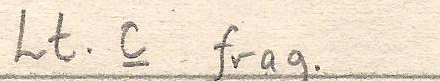
\includegraphics[width=0.3\textwidth]{../images/data_samples/canine.png} & Lt. \underline{C} frag. \\
        \hline
        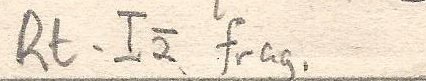
\includegraphics[width=0.3\textwidth]{../images/data_samples/lowjawincisor.png} & Rt. I$\bar{\check{2}}$ frag. \\
        \hline
        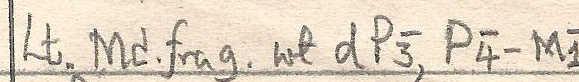
\includegraphics[width=0.3\textwidth]{../images/data_samples/multipleteeth.png} & Lt. Md. frag. wt dP$\check{\bar{3}}$, P$\check{\bar{4}}$-M$\check{\bar{1}}$\\
        \hline
        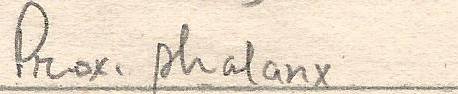
\includegraphics[width=0.3\textwidth]{../images/data_samples/nontooth.png} & Prox. phalanx \\
        \hline
        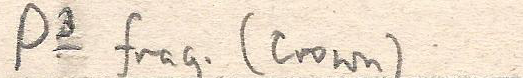
\includegraphics[width=0.3\textwidth]{../images/data_samples/smudged.png} & P$\hat{\underline{\text{3}}}$ frag. (Crown) \\
        \hline
        
\includegraphics[width=0.3\textwidth]{../images/data_samples/underlinedx.png} & ? M$\hat{\underline{\text{x}}}$ frag. \\
        \hline
    \end{tabular}
    \caption{Samples of input images and their corresponding labels.}
    \label{table:input_images}
\end{table}

\subsubsection{Data preprocessing}

\subsection{Methods}

\subsubsection{Encoding prior knowledge}

\section{results}

\section{conclusion}

\printbibliography

\end{document}